\documentclass[nopagenumber,9pt]{beamer}

\mode<presentation> {
  \usetheme[]{CambridgeUS}
  %\useoutertheme{shadow}
  \setbeamercovered{transparent}
  \usecolortheme{seahorse}
%\usecolortheme{sidebartab}
%  \usefonttheme{structurebold}
  \useinnertheme{default}
\useinnertheme{rounded}
}
\usepackage{nicefrac}
\RequirePackage{amsmath,amsfonts,amsthm}

\usepackage{float}
\usepackage[english]{babel}
\usepackage{amsmath}
\usepackage[utf8]{inputenc}
\usepackage{times}
\usepackage{url}
\usepackage[T1]{fontenc}
%\usepackage{multirow}
\usepackage{color}
\newcommand{\mb}[1]{\mathbf{#1}}
\usepackage{graphicx}
\graphicspath{{./figure/}}

\usepackage[ruled,vlined]{algorithm2e}
\usepackage{xcolor,colortbl}
\usepackage{rotating}
\usepackage{multirow}

\usepackage{tikz}
\usepackage{ulem}


\usetikzlibrary{calc,shapes,backgrounds,arrows,automata,shadows,positioning}

\usepackage{xcolor,pifont}
\definecolor{lgreen}{RGB}{188,214,49}
\definecolor{dgreen}{RGB}{139,172,100}
%pour biblio en bleu
\hypersetup{
  colorlinks = true,
  linkcolor = black
}
\makeatletter
\let\@mycite\@cite
\def\@cite#1#2{{\hypersetup{linkcolor=blue!60!black}[{#1\if@tempswa , #2\fi}]}}
\makeatother

\newcommand{\argmax}[2]{% 
\smash{\mathop{{\rm argmax}}\limits_{#1}}\,#2} 

\newcommand{\ZR}[1]{Z^{I}_{#1}}
\newcommand{\ZL}[1]{Z^{O}_{#1}}
\newcommand{\bZR}{\mathbf{Z}^{I}}
\newcommand{\bZL}{\mathbf{Z}^{O}}
\newcommand{\XR}[1]{Y^{I}_{#1}}
\newcommand{\XL}[1]{Y^{O}_{#1}}
\newcommand{\bXR}{\bY^{I}}
\newcommand{\bXL}{\bY^{O}}
\newcommand{\nbr}{n_I}
\newcommand{\nbl}{n_O}
\newcommand{\aff}{A}
\newcommand{\QR}{K_I}
\newcommand{\QL}{K_O}
\usepackage{tikz}
%\usetikzlibrary{calc,shapes,backgrounds,arrows,automata,shadows,positioning}
\usetikzlibrary{arrows,shapes,positioning,shadows,trees,calc,backgrounds,automata,positioning}



\tikzset{
  basic/.style  = {draw, text width=3cm, font=\sffamily, rectangle},
  root/.style   = {basic, rounded corners=2pt, thin, align=center,
                   fill=green!30},
  level 2/.style = {basic, rounded corners=6pt, thin,align=center, fill=green!60,
                   text width=8em},
  level 3/.style = {basic, thin, align=left, fill=pink!60, text width=3.5cm}
}


% pour tickz multilevel
\definecolor{redorg}{RGB}{215,48,39}
\definecolor{orangeorg}{RGB}{253,174,97}
\definecolor{blueind}{RGB}{69,117,233}
\definecolor{cyanind}{RGB}{116,173,209}
\definecolor{greenind}{RGB}{112,130,56}



% pour epidemio
%\usepackage[dvipsnames]{xcolor}
%\newcommand*\circled[1]{\tikz[baseline=(char.base)]{
%            \node[shape=circle,draw,inner sep=1pt] (char) {#1};}}

% \xdefinecolor{nice_green}{named}{Emerald}
% \xdefinecolor{nice_red}{named}{WildStrawberry}

\newcommand{\MA}{\bY}
\newcommand{\Xn}{\MA}
\newcommand{\MAO}{\MA^\text{\rm o}}
\newcommand{\MAM}{\MA^\text{\rm m}}

\newcommand{\blue}{\textcolor{myblue}}
\definecolor{myblue}{RGB}{0,56,115}
\newcommand{\bR}{\mathbf{R}}

%variables vectorielles
\newtheorem{proposition}{Proposition}
\newcommand{\I}{\mathbb{I}}
\newcommand{\E}{\mathbb{E}}
\renewcommand{\P}{\mathbb{P}}
\newcommand{\R}{\mathbb{R}}
\newcommand{\bs}{\boldsymbol}
\newcommand{\bbeta}{\boldsymbol{\beta}}
\newcommand{\balpha}{\boldsymbol{\alpha}}
\newcommand{\btheta}{\boldsymbol{\theta}}
\newcommand{\bY}{\mathbf{Y}}
\newcommand{\bX}{\mathbf{X}}
\newcommand{\bZ}{\mathbf{Z}}
\newcommand{\by}{\mathbf{y}}
\newcommand{\bz}{\mathbf{z}}
\newcommand{\ba}{\mathbf{a}}
\newcommand{\bx}{\mathbf{x}}
\newcommand{\bh}{\mathbf{h}}
\newcommand{\bb}{\mathbf{b}}
\newcommand{\bB}{\mathbf{B}}
\newcommand{\bM}{\mathbf{M}}
\newcommand{\bphi}{\boldsymbol{\phi}}
\newcommand{\bpsi}{\boldsymbol{\psi}}
\newcommand{\bpi}{\boldsymbol{\pi}}
\newcommand{\btau}{\boldsymbol{\tau}}
\newcommand{\Ecal}{\mathcal{E}}
\newcommand{\GP}{\mathcal{GP}}
\newcommand{\bxi}{\boldsymbol{\xi}}
\newcommand{\brho}{\boldsymbol{\rho}}
\newcommand{\bgamma}{\boldsymbol{\gamma}}
\newcommand{\bsigma}{\boldsymbol{\sigma}}

\newcommand{\bneta}{\boldsymbol{\eta}}
\newcommand{\logit}{\textrm{logit}}

\newcommand{\M}{\mathcal{M}}

\newcommand{\bxf}{\bx^e}
\newcommand{\bXf}{\bX^e}
\newcommand{\nf}{n_e}
\newcommand{\Df}{D^e}
%\newcommand{\GP}{GasP}
%fielddata
\newcommand{\yf}{y^e}
\newcommand{\xf}{x^e}
\newcommand{\byf}{\by^e}
\newcommand{\byfsuper}[1]{\by^{e,{#1}}}
\newcommand{\bm}{\mathbf{m}}
\newcommand{\bV}{\mathbf{V}}
\newcommand{\ind}{\mathbb{I}}



\newcommand{\blambda}{\boldsymbol{\lambda}}
\newcommand{\bepsilon}{\boldsymbol{\epsilon}}
\def\ee{{\mathbb E}}

\newcommand{\ms}[1]{\boldsymbol{#1}}
\newcommand{\dd}{\mathrm{d}}
\newcommand{\Scal}[3]{<#2,#3>_{#1}}

\newcommand{\Norm}[2]{||#2||_{#1}}

\renewcommand{\sc}{\fontfamily{pag}\fontseries{m}\fontshape{sc}\selectfont}
\renewcommand{\textsc}[1]{{\sc#1}}

\newcommand{\citemano}[1]{\textcolor{dgreen}{#1}}


\newcommand{\adj}{A}


\newcommand\MF{{\mathfrak{M}}}

\title[Habilitation Defense]{Statistical Contribution to Uncertainty Quantification\\  and the Analysis of Networks}

%titre premiere page

\subtitle{Soutenance en vue de l’obtention
du Diplôme d’Habilitation à Diriger les Recherches}

\author[P. Barbillon]{ Pierre \textsc{Barbillon}}
\bigskip

\date{December, 10. 2020}

\subject{Séminaire}



\AtBeginSection[] {
 \begin{frame}<beamer>
   \frametitle{Outline}
   \tableofcontents[currentsection]
  \end{frame}
}

\AtBeginSubsection[] {
\begin{frame}<beamer>
   \frametitle{Outline}
   \tableofcontents[currentsection,currentsubsection]
 \end{frame}
}


\begin{document}

\begin{frame}
\titlepage
%\includegraphics[scale=.12]{AgroParisTech_-_logo.PNG}
%\vspace{-1.5cm}
%\begin{flushright}
% \includegraphics[scale=.1]{Logotype-INRA-transparent.png}
% \end{flushright}
\vspace{-1cm}
\centering
\begin{tabular}{ccc}
 \includegraphics[scale=.08]{LogoUPSaclay.jpg}&
  \includegraphics[scale=.18]{logoAgroParisTech.jpg}&
   \includegraphics[scale=.1]{LogoINRAE.jpg}
\end{tabular}


\end{frame}



\begin{frame}
 \frametitle{Education and Work Experience}

% \begin{tabular}[t]{@{}p{.15\linewidth}|p{.8\linewidth}}    
%     since 9/2011&Associate Professor at AgroParisTech\\
% & Moel
%     \end{tabular}\medskip

 
 
 \begin{beamerboxesrounded}{Ph.D. Thesis}
\begin{tabular}[t]{@{}p{.15\linewidth}|p{.8\linewidth}}    
    2007-2010&\textit{Kernel interpolation methods for estimating
expensive black box function}\\
& Defended in 2010 at Université Paris Sud\\
& Supervisor: Jean-Michel Marin
    \end{tabular}\medskip
  
 \end{beamerboxesrounded}

 
 \bigskip
 

 

 \begin{beamerboxesrounded}{Positions}
\begin{tabular}[t]{@{}p{.15\linewidth}|p{.8\linewidth}}    
    since 9/2011&Maître de conférence / Associate Professor at AgroParisTech\\
& UMR MIA-Paris, AgroParisTech/INRAE, Université Paris Saclay.
    \end{tabular}\medskip

  
\begin{tabular}[t]{@{}p{.15\linewidth}|p{.8\linewidth}}    
    2018-2019&Visiting Research Fellow at SAMSI\\
    & MUMS program (Model Uncertainty: Mathematical and Statistical)\\
    & Agreenskills+ Grant.
  \end{tabular}\medskip
 \end{beamerboxesrounded}
  
  
  
  
\end{frame}




\begin{frame}
\frametitle{Outline}
 \tableofcontents
\end{frame}



\section{Overview }


	\begin{frame}{Scientific Question: Impact of the Social network on a seed circulation model}
		\frametitle{}
		In collaboration with M. Thomas, I Goldringer, F. Hospital and S. Robin. \cite{barbillon2015network}
		\begin{columns}
			\begin{column}{5cm}
				\begin{center}
					\begin{figure}
						\includegraphics[scale=0.3]{2_levels_networks_illus.pdf}
					\end{figure}	
					\label{M. Thomas}
				\end{center}
			\end{column}
			\begin{column}{5cm}	
		\begin{exampleblock}{Assumption}
			Seed exchange networks are nested within advice networks
		\end{exampleblock}
			\end{column}	
		\end{columns}
		\begin{block}{ Refined question}
			 To what extent do the topological properties of the advice network influence the persistence of seed varieties?		
		\end{block}
		
		
	\end{frame}


	

	\begin{frame}
	 \frametitle{Dynamic Model}
	 \begin{minipage}{0.60\linewidth}
	 \vspace{-1cm}
	  \textbf{Time $t$:} n nodes=farmers growing the seed (blue nodes) not growing the seed (orange nodes)\\
	  
	  \vspace{.5cm}
	  
	  For going from time $t$ to time $t+1$:\\
	  
	  \vspace{.2cm}
	  
	  \textbf{Extinction Step:} independently with probability $e$,\\
	  
	  \vspace{1cm}
	  
	  \textbf{Colonization Step:} from a non-empty neighbor (according to the network) with probability $c$.
	 \end{minipage}\hfill
	 \begin{minipage}{.36\linewidth}
	  \centering
	\includegraphics[scale=.1]{gent.pdf}\\
\includegraphics[scale=.1]{gentextin.pdf}\\
\includegraphics[scale=.1]{gent1.pdf}
	 \end{minipage}

	 
	 $\Rightarrow$ Markov Chain with $2^n$ states


	 
	\end{frame}


	\begin{frame}
	 \frametitle{Analysis of a computer model / simulator}
	 
	 Outputs of the computer model: $(\bZ_t\in\{0,1\}^n)_{0\le t\le T}$
	 
	 \begin{figure}[h!]
\centering
\begin{tabular}{cc}
 \includegraphics[scale=0.15]{e0_25c0_01d0_3.pdf}&
 \includegraphics[scale=0.15]{espe0_25c0_01d0_3.pdf}
\end{tabular}
	\caption{Probability of persistence (left) and  mean number of occupied patches (right), 
in varying $t$ generations for different network topologies and fixed $e$ and $c$.}
\label{figdifftopo}
\end{figure}
	 
	 
	 \begin{beamerboxesrounded}{Sensitivy Analysis}
 
 $$\underbrace{e, \ c ,\ G}_{inputs} \rightarrow\fbox{Dynamic Model}\rightarrow \underbrace{\P(T_0> t),\ \E(\#Z_{t})}_{outputs}   \,,$$
based on numerical runs of the dynamic model for well-chosen combinations of inputs.
 
\end{beamerboxesrounded}


	\end{frame}


	
	
	
	\begin{frame}
	 \frametitle{Network input}
	 
	 
	 
	  \begin{figure}
  \begin{center}
\includegraphics[scale=.1]{networksMAJ.jpeg}
 \end{center}
\caption{Networks with $100$ nodes and $247$ edges according to Erd\H{o}s-R\'enyi model (\textbf{A}), community model simulated from the Stochastic Block Model \citemano{[NS01]} (\textbf{B}),
lattice model (\textbf{C}), preferential attachment model with power 1 (\textbf{D}) and power 3 (\textbf{E}). %The size of a node is 
%proportional to its degree.
}
\label{figtoponet}
\end{figure}
	 
	 \begin{beamerboxesrounded}{G: Network Input $\rightarrow$ 2 parameters}
	  \begin{itemize}
	   \item $d$ density ($\sim$ number of edges),
	   \item Topology: the way the edges are distributed across nodes.
	  \end{itemize}

	 \end{beamerboxesrounded}

	 
	 
	\end{frame}


	
	% presentation des travaux en donnant soit les refs soit le nombre d epapier sur les sujets
	
	\begin{frame}
	 \frametitle{Questions relative to Uncertainty Quantification}
	 
	 % en italique ce que c'est ici
	 \begin{itemize}
	  \item Sensitivity analysis \cite{barbillon2015network,ferrer,lecarpentier2019walter}.\\
	   \textit{e.g. impact of the inputs $e,c,G$ on the outputs.}
	   \smallskip
	   
	  \item Dimension of inputs, outputs \cite{ferrer}.\\
	  \textit{e.g. $t\mapsto\P(T_0> t)$ (functional output).} 
	  
	  	   \smallskip

	  \item Deterministic or Stochastic simulator \cite{stosim}\\
	  \textit{e.g. Simulated stochasticity within the computer model}.

	  	   \smallskip

	  \item Calibration and inverse problem \cite{barbillondamblin,metamodmix,carmassiPV}.\\
	  \textit{e.g. estimate $e$, $c$ from the real-world observations of time-series of 0/1 states for each farm over time: $(\bZ_t)_{0\le t\le T}$.}
	   \smallskip

	  
	  \item Validation of the simulator and post-processing \cite{damblin2016bayesian,kaniav,courbariaux2017water,courbariaux2019post}.\\
	  \textit{e.g. do values for $e$, $c$ make the simulator mimic precisely enough the real world process?}
	 \end{itemize}

	 
	 
	\end{frame}

	
	
	% faire 2 slides en grisant ce qu'on ne prendre pas le temps de présenter plus en détail ???
	
	\begin{frame}
	 \frametitle{Questions relative to the analysis of networks}
	 
	 \begin{itemize}
	  \item Impact of the structure of a network \cite{barbillon2015network}.
	  \medskip
	  
	  \item Inference of the network when status are observed over time \cite{barbillon2019epidemiologic}\\
	  \textit{e.g. estimate the contact network from real-world observations of time-series of 0/1 states for each farm over time: $(\bZ_t)_{0\le t\le T}$.}
	  \medskip
	  
	  
	  \item From the observation of a network, can we unravel its structure? \smallskip
	  
	  \textit{e.g. From some interviews with farmers, is it possible to detect specific communities of farmers, particular farmers who are central in the network...}
	  
	  \begin{itemize}
	   \item Comparison of local patterns \cite{thomasInventory}.
	\smallskip
	
	
	   \item Unravelling the structure in spite of the observation process \cite{tim,missSBM}.\smallskip
	   
	   \item Multilayer networks \cite{barbillon2017stochastic,lazega2016effects,bar2018block,chabert2019stochastic}. 
	  \smallskip
	  
	  \end{itemize}

	  
	  
	  
	 \end{itemize}

	 
	\end{frame}
	
	
	
\section{Uncertainty Quantification}




\subsection{Statistical Framework}
\begin{frame}
 \frametitle{Calibration and Validation of a Simulator / Computer Model}
 
 \textbf{Simulator:}
$f:(\bx,\btheta)\mapsto f(\bx,\btheta)\in \mathbb{R} $ where\\
\medskip
\begin{itemize}
  \item \textbf{input variables}: $\bx\in  \mathbb{X}\subset\mathbb{R}^p$ observable  in the real world,
  \smallskip
  \item \textbf{simulator parameters}: $\btheta\in \Theta\subset\mathbb{R}^q$ non-observable parameters, required to run the simulator.
\smallskip
  
\end{itemize}

  \bigskip
  
%   \textbf{Emulation:}
%  $f$ is long-time running, so it may need to be emulated:
%  $$$$
%   
  
  
  \textbf{Calibration:}\\
  If $f$ simulates 
  the real-world phenomenon $f^R$:   
  calibration consists in finding the ``best'' or ``true'' $\btheta^*$ from real observations / field data such that
  $$f^R(\bx)\approx f(\bx,\btheta^*)\,.$$

  
  \textbf{Validation:}\\
  Is the approximation $f^R(\bx)\approx f(\bx,\btheta^*)$ accurate enough with respect to the intended use?
  
  
  
\end{frame}



\begin{frame}
 \frametitle{Statistical Framework \citemano{[KO01]}}

\textbf{Data:}

\begin{enumerate}
 \item DoNE: Design of Numerical Experiments: $D=\{(\bx_1,\btheta_1),\ldots,(\bx_N,\btheta_N)\}$  %(space-filling or optimize with respect to a given goal: rare event, global optimization)
with corresponding evaluations of the computer model (time-consuming):
$$f(D)=\{f(\bx_1,\btheta_1),\ldots,f(\bx_N,\btheta_N)\}\,.$$ 
 
 
 \item DoFE: Design of Field Experiments: $\Df=\{\bxf_1,\ldots,\bxf_{\nf}\}$ with corresponding noisy observation of $f^R$:$$\byf=\{y_1=f^R(\bxf_1)+\epsilon_1,\ldots,y_n=f^R(\bxf_{\nf})+\epsilon_{\nf}\}\,.$$ 
\end{enumerate}



 
 
 
\smallskip

\textbf{Model:}\quad
$\forall 1\le i \le \nf,\quad \yf_i = f(\bxf_i,\btheta) + \delta(\bxf_i) +\epsilon_i$
where:

\smallskip
\begin{itemize}
 \item $f$ is emulated via a GP Emulator \citemano{[SWMW89]}: $f\sim \mathcal{GP}(m(\cdot),\sigma_F^2C(\cdot,\cdot))$,\\ $f|f(D)\sim \mathcal{GP}$ is the emulator/surrogate/metamodel,
 \item $\delta$ the discrepancy modeled as a GP: $\delta\sim \mathcal{GP}(0,\sigma_\delta^2C_\delta(\cdot,\cdot))$,
 \item $\epsilon\overset{iid}{\sim}\mathcal{N}(0,\sigma_{\epsilon}^2)$ are measurement errors.
\end{itemize}


%\smallskip




\end{frame}


\subsection{Some contributions}


\begin{frame}
 \frametitle{Adaptive Design of experiments for the calibration goal}
 In collaboration with G. Damblin (Ph.D. Thesis), M. Keller and É. Parent \cite{barbillondamblin} 
 

 \bigskip
\textbf{Calibration:} estimate $\btheta$ via MCMC algorithms.
 
 \smallskip
 Choice of $D$ to make the posterior distribution $\pi_2$ as close as possible to $\pi_1$: 
 \begin{eqnarray*}
 \pi_1(\btheta|\byf)&\propto& \ell(\btheta;\byf) \cdot\pi(\btheta)\, \rightarrow \text{depends on }f\\
 \pi_2(\btheta|\byf,f(D))&\propto& \ell_D(\btheta;\byf)\cdot\pi(\btheta)\, \rightarrow \text{where emulator replaces } f.\\
\end{eqnarray*}
 
 
 \medskip
 \textbf{Heuristics:} important to have a reliable emulator when $\pi_1(\btheta|\byf)$ is high:
 it leads to maximize 
 $$SS(\btheta)=\Vert \byf-(f(\bxf_i,\btheta))_{1\le i\le \nf} \Vert^2$$
 by adapting the Expected Improvement of \citemano{[JSW98]} in order to maximize $SS$:
%  \begin{equation*}
% \label{EI_calib}
% EI_{k}(\btheta)=\E \left[\big(s_k-SS_{k}(\btheta)\big)\mathbb{I}_{SS_{k}(\btheta)\leq s_k}\right]\,\,\,\in\,\,\,[0,s_k],
% \end{equation*}
% where 
% \begin{itemize}
% \item $s_k$ current minimum,
% \item 
% $ SS_{k}(\btheta)=||\byf-F^{D_k}({\btheta})||^{2}\,.$
% \end{itemize}

\smallskip
\begin{itemize}
 \item maximization of a function of $f$ rather than $f$ directly,
 \smallskip
 \item we obtain a sequential design adapted to calibration.
\end{itemize}


\end{frame}


\begin{frame}
 \frametitle{Illustration}

 \begin{minipage}{.5\textwidth}
 Sequential design adapted to calibration :
 \includegraphics[scale=0.3]{restricted_maximin9_seq.pdf}
 \begin{itemize}
  \item $\bullet$ starting space-filling design,
  \item \color{red}$\star$ \color{black} points added sequentially.
 \end{itemize}

 \end{minipage}\hfill
\begin{minipage}{.45\textwidth}
Better performance than space-filling DoNE:
\begin{itemize}
 \item on synthetic example according to the Kullback-Leibler discrepancy \cite{barbillondamblin},
 \item and for prediction in a photovoltaic simulator \cite{carmassiPV} (part of the Ph.D. Thesis of M. Carmassi). 
\end{itemize}
 
 \end{minipage}

 
\end{frame}

% 
% \begin{frame}
%  \frametitle{Inverse Problem}
%  In collaboration with C. Barthélémy and A. Leclercq-Samson \cite{metamodmix}. 
%  
%  \bigskip
%  
%  Computer model within a \textbf{mixed-model} (e.g. compartment model in pharmacokinetics)\\
% $ \forall i=1,\ldots,\nf;\ j=1,\ldots,n_i:$
% 
% \vspace{-.3cm}
%   \begin{equation*}\label{eq:MixedModel}
% \begin{array}{lcl}
%  \yf_{ij} &= &  f (\bxf_{ij}, \psi_i) + \, \epsilon_{ij}, \quad  \epsilon_{ij} \sim_{iid} \mathcal{N}(0,\sigma_\epsilon^2)\\
%  \psi_i &\sim_{iid}&    \mathcal{N}(\mu,\Omega) \quad \text{individual parameters sampled in a population distribution}
% \end{array}\,.
%  \end{equation*}
%  
%  The goal is to estimate jointly $\btheta=(\mu,\Omega)$ and $\sigma_\epsilon^2$.
% 
%  \bigskip
%  \begin{itemize}
%   \item SAEM algorithm because of unobserved $\psi_i$s simulated by an MCMC algo \citemano{[KL04]} ,
%   \item Replacement of $f$ by its emulator in the likelihood: 
%   $\ell(\btheta,\sigma_\epsilon^2;\byf)\rightarrow \ell_D(\btheta,\sigma_\epsilon^2;\byf)$,
%   \item Computational burden in the MCMC sampling: cov matrix of the emulator $\bV_{e|f(D)}$,
%   \item Alleviate this burden by neglecting non-diagonal terms in $\bV_{e|f(D)}$,
%   \item Convergence of SAEM algorithm toward maximum of $\ell_D(\btheta,\sigma_\epsilon^2;\byf)$ and control on
%   $$|\ell(\btheta,\sigma_\epsilon^2;\byf)-  \ell_D(\btheta,\sigma_\epsilon^2;\byf)|$$
%  \end{itemize}
% 
%  
% 
%  
%  \end{frame}
%  
% \begin{frame}
%  \frametitle{Inverse Problem}
%  In collaboration with C. Barthélémy and A. Leclercq-Samson \cite{metamodmix}. 
%  
%  \bigskip
%  
%  Costly computer model within a \textbf{mixed model} (example in a compartment model in pharmacokinetics)
%  
% 
%   \begin{equation*}\label{eq:MixedModel}
% \begin{array}{lcl}
%  \yf_{ij} &= &  f (\bxf_{ij}, \psi_i) + \, \epsilon_{ij}, \quad  \epsilon_{ij} \sim_{iid} \mathcal{N}(0,\sigma_\epsilon^2)\\
%  \psi_i &\sim_{iid}&    \mathcal{N}(\mu,\Omega) 
% \end{array}\,.
%  \end{equation*}
%  
%  The goal is to estimate jointly $\btheta=(\mu,\Omega)$ and $\sigma_\epsilon^2$.
%  
%  
%  \bigskip
%  
%  \only<1>{ \textbf{Likelihood:}
%  
%  
%  \begin{equation*}\label{eq:Likelihood}
%  \begin{array}{lll}
% &&\ell(\btheta,\sigma_\epsilon^2;\byf) = \int \ell(\btheta,\sigma_\epsilon^2,\bpsi\, ; \byf)\,d\bpsi 
% = \prod_{i=1}^{\nf}\int \pi(\byf_i|\psi_i,\sigma_\epsilon^2) \pi(\psi_i| \btheta) d\psi_i\\
% &=&\prod_{i=1}^{\nf} \int 
% \Bigg\{\pi(\psi_i| \btheta)\frac{1}{(2\pi \sigma_\epsilon^2)^{n_i/2}}\\
% &&\times
% \exp\left(-\frac{1}{2} (\byf_i-f(\bxf_i,\psi_i))^t(\sigma_\epsilon^2 I_{n_i})^{-1}(\byf_i-f(\bxf_i,\psi_i)) \right) 
%  d\psi_i\Bigg\}
%  \end{array}\,,
%  \end{equation*}}
% 
%  %\bigskip
%  
%  \only<2>{ \textbf{Likelihood with \color{red}an emulator\color{black}:}
%   \begin{equation*}\label{eq:completeMetaLikelihood}
% \begin{array}{lll}
%  \ell_D(\btheta,\sigma_\epsilon^2;\byf)&=&
% %&&=\int p(\bpsi;\btheta) \ell_D(\by|\bpsi;\btheta)d\bpsi\,,\nonumber\\
% \int \Bigg\{ \pi(\psi_i| \btheta)\;  \frac{1}{(2\pi)^{n_{tot}/2}\color{red}|\bV_{e|f(D)}|^{1/2}\color{black}}\\
% &&\exp\bigg(-\frac{1}{2}(\byf-\color{red}\bm_{e|f(D)}\color{black})^t(\color{red}\bV_{e|f(D)}\color{black})^{-1}
% (\byf-\color{red}\bm_{e|f(D)}\color{black}) \bigg)\,d\bpsi
% \Bigg\}\,,
% \end{array}
% \end{equation*}
%  where $n_{tot}=\sum_{i=1}^{\nf} n_i$, 
%  $\bm_{e|f(D)} = (m_D(\bxf_{ij},\psi_i))_{1\le i\le \nf,1\le j\le n_i} $  
%  and $\bV_{e|f(D)}
%  =\sigma_\epsilon^2 I_{n_{tot}}+(C_D((\bxf_{ij},\psi_i),(\bxf_{i'j'},\psi_{i'})))_{1\le i,i'\le \nf,1\le j,j'\le n_i}$.
%  }
% \end{frame}
% 
% 
% 
% 
% \begin{frame}
%  \frametitle{Estimation}
%  
%  \begin{algorithm}[H]
% At iteration $k$, given the current values of the estimators  $\hat\btheta^{(k-1)}, \hat \sigma_\epsilon^{2\,(k-1)}$:
% \caption{SAEM-MCMC algorithm \citemano{[KL04]}}
% \begin{itemize}
% \item[] \textbf{Simulation step:} Update   $\psi_i^{(k)}$  with $m$ iterations of an MCMC procedure with $\pi_D(\psi_i|\byf_i; \widehat{\theta}^{(k-1)},\bpsi_{-i},\sigma_\epsilon^2)$ as stationary distribution.
% \item[] \textbf{Stochastic Approximation step:} %update   the sufficient statistics $
% 	%s_{k,1}$, $s_{k,2}$ and $s_{k,3}$ 
% 	$s_{k,l}=s_{k-1,l} + \gamma_k \,\left(S_{l}(\byf,\bpsi^{(k)}) -s_{k-1,l}\right)$
% \item[] \textbf{Maximization step:} %  update the population parameters
% 	%\begin{eqnarray*}
% 	$\widehat{ \mu}^{(k)}  =  \frac{s_{k,1}}{\nf}, \quad	 \widehat{\Omega}^{(k)}  =  \frac{s_{k,2}}{\nf}-\frac{s_{k,1}\, s_{k,1}^t}{\nf^2}, \quad 
% 	\widehat{\sigma}_\epsilon^{2\,^{(k)}}  =  \frac{s_{k,3}}{n_{tot}}\,.$
% 	%\end{eqnarray*}
% 		\end{itemize} 
% \end{algorithm}
%  
%  $\Rightarrow$ Alleviate the simulation step by neglecting non-diagonal terms in $\bV_{e|f(D)}$.
%  
%  \begin{proposition}
% Under some standard assumptions, we have convergence of the SAEM estimates and 
%  $$
%  |\ell(\btheta,\sigma_\epsilon^2;\byf)-  \ell_D(\btheta,\sigma_\epsilon^2;\byf)|\le  %\hat
%  \text{Cst}_{\byf}\frac{n_{tot}}{\sigma_\epsilon^{n_{tot}+2}}  G_C(h_D)\,
% $$
% where $h_D$ is the covering distance associate with the DoNE and $G_C$ is a function decreasing to $0$ with $h_D\rightarrow0$. 
% \end{proposition}
%  
%  
% \end{frame}
% 




\begin{frame}
 \frametitle{Validation as hypotheses testing}
 
 In collaboration with G. Damblin, K. Kamary, É. Parent, M. Keller \cite{damblin2016bayesian,kaniav}.
 
 \bigskip
 
 
  Under the simplifying assumption: $f(\bx,\btheta)=g(\bx)^T \btheta$, we compare
 
 \begin{align*}
 \mathcal{H}_0:\quad & \yf_i = f(\bxf_i,{\btheta}) + \epsilon_i\,,\\
 \mathcal{H}_1:\quad & \yf_i = f(\bxf_i,{\btheta}) + \delta(\bxf_i) + \epsilon_i\,.\\
\end{align*}
% Under $\mathcal{H}_1$, we assume that $\delta\sim\mathcal{GP}(0,\sigma^2_\delta C_\delta(\cdot,\cdot))$ and under $\mathcal{H}_0$ and $\mathcal{H}_1$ we still assume that  $\epsilon_i\overset{i.i.d.}{\sim}\mathcal{N}(0,\sigma_\epsilon^2)$.
%  
 
 \textbf{Bayes Factor}
 $$B_{0,1}(\byf):=\frac
{\int \ell_{\mathcal H_0}(\btheta ,\sigma_\epsilon^2;\byf )\pi(\btheta ,\sigma_\epsilon^2)d \btheta d\sigma_\epsilon^2}
{\int \ell_{\mathcal H_1}(\btheta ,\sigma_\epsilon^2,\sigma_\delta^2,\phi_\delta;\byf )\pi(\btheta ,\sigma_\epsilon^2,\sigma_\delta^2,\phi_\delta)d \btheta d\sigma_\epsilon^2d\sigma_\delta^2d\phi_\delta}\,.$$
$\Rightarrow$ Need for compatible prior distributions, intrinsic Bayes Factor. 


\bigskip


\textbf{Mixture Model}
 \begin{equation*}\label{eq:mixture}
\mathcal M_\alpha: \yf_i\overset{ind.}{\sim} \alpha \left(\ell_{\mathcal H_0}(\btheta, \sigma_\epsilon^2;\yf_i)\right)+(1-\alpha)\left(\ell_{\mathcal H_1}(\btheta, \sigma_\epsilon^2, \delta;\yf_i)\right)\,,
\end{equation*}
 as in \citemano{[KMRR14]} where $\delta$ is assumed to be latent.
 
\end{frame}



\begin{frame}
\frametitle{Simulation results}
 \begin{figure}
 \centering
%  \includegraphics[width=0.45\textwidth]{figures/const_30_unif_prior.png}
% \includegraphics[width=0.45\textwidth]{figures/lin_30_unif_prior.png}
\begin{tabular}{c@{\hspace{.03mm}}c@{\hspace{1ex}}}
 \rotatebox{90}{\hspace{1.5cm}Bayes Factor $B_{0,1}$}&\includegraphics[width=0.5\textwidth]{poly_30_unif_prior.png} \\
 & {\hspace{.5cm} Range parameter of the discrepancy}
\end{tabular}
\caption{Bayes factor computations over $100$ simulated datasets of size $\nf=30$.} %The x-value gives  the range parameters of the exponential kernel used to generate the discrepancy.} %The simulator is a  $f(\bx)=(1,x,x^2) (\theta_0,\theta_1,\theta_2)^t $. }
\label{figIBF}
\end{figure}

 
\end{frame}


\subsection{Perspectives in UQ}


\begin{frame}
 \frametitle{Selecting the active variables in the discrepancy}
In collaboration with A. Forte and R. Paulo.
 \bigskip
 
 %A classical choice is the power exponential kernel:
Power exp. kernel $C_{\delta}(\bx,\bx')= \prod_{j=1}^d \exp\left(-\frac{|x_j-x_j'|^\alpha}{\phi_j}\right) = \prod_{j=1}^d \rho_j^{2^\alpha |x_j-x_j'|^\alpha}$

 where 
 \begin{itemize}
  \item $1\leq\alpha\leq2$ is usually fixed,
  \item Reparametrization of $\phi_j\in(0,\infty)$ in  $\rho_j\in[0,1]$ (\citemano{[LBH+06]}). 
 \end{itemize}
 
 
 
   \begin{minipage}{.5\textwidth}
%  \begin{equation*}
%  \pi(\brho\mid \bgamma) = \prod_{i=1}^p \left[\gamma_i\ I_{[0,1]}(\rho_i) + (1-\gamma_i)\ \delta_1(\rho_i)\right] 
%  \end{equation*}

\medskip

\textbf{Prior on $\brho$:}
$$\pi(\brho|\bgamma)= \prod_{j=1}^d \Big(\gamma_j \mathcal{U}[0,1](\rho_j)  +(1-\gamma_j)\mathcal{B}e(\nu,1)(\rho_j)\Big) $$

with $\bgamma \in \{0,1\}^p$.% $\gamma_i\overset{iid}{\sim}b(\tau)$.

\begin{itemize}

\item $\gamma_j=1\Leftrightarrow\mathcal{B}e(1,1)=\mathcal{U}[0,1]$ active variable,
 \item $\gamma_j=0$ encourages inert variable for $\nu>>1$.
 %\item either smooth version of spike-and-slab priors.
\end{itemize}
 \end{minipage}
 \begin{minipage}{.45\textwidth}
 \centering
 \includegraphics[scale=.2]{prior.pdf}
 \end{minipage}
 
\end{frame}


\begin{frame}
\frametitle{Model Selection and Variable Selection} 
 \begin{beamerboxesrounded}{Model definition}
 $\M_{\bgamma}$: likelihood $\ell\big(\brho,\bneta;\by \big)$ and
\textbf{prior}: $\pi(\brho|\bgamma)\cdot \pi(\bneta)$. ($\bneta=(\btheta,\sigma^2_\epsilon,\sigma^2_\delta)$).\\
$\rightarrow$ $2^p$ possible models ($\forall j,\ \gamma_j\in\{0,1\}$).
  \end{beamerboxesrounded}

 
 
 \bigskip
 
 \textbf{Model posterior probability:}
 $\P(\M_{\bgamma}|\by) \propto \int \ell\big(\brho,\bneta;\by \big) \pi(\brho|\bgamma) \pi(\bneta) d\brho d\bneta\cdot \P(\M_{\bgamma})$. 
 \\
 $\Rightarrow$ Large marginal likelihood if good agreement between data and priors.
 
 
 \bigskip
 
 
 \textbf{Computation of posterior probabilities:} by importance sampling from a unique MCMC algorithm sampled in $\M_{\bgamma=1}$: $ \left(\brho^{(k)},\bneta^{(k)}\right)_{k=1,\ldots,N}$

 $$BF(\M_{\bgamma},\M_1) \approx \frac{1}{N}\sum_{k=1}^N \frac{\ell\big(\brho^{(k)},\bneta^{(k)};\by\big)\pi\big(\brho^{(k)}|{\bgamma}\big)\pi\big(\bneta^{(k)}\big)}{\ell\big(\brho^{(k)},\bneta^{(k)};\by\big)\pi\big(\brho^{(k)}|\boldsymbol{1}\big)\pi\big(\bneta^{(k)}\big)}=\frac{1}{N}\sum_{k=1}^N\frac{\pi\big(\rho_1^{(k)},\ldots,\rho_d^{(k)}|{\bgamma}\big)}{\pi\big(\rho_1^{(k)},\ldots,\rho_d^{(k)}|\boldsymbol{1}\big)}\,.$$
 
 \textbf{Variable selection:} 
For each variable, posterior inclusion probabilities computed on the basis of the posterior probabilities for models:

$$P(x_j \text{ is active}|\by)= \sum_{\bgamma:\gamma_j=1}\P(\M_{\bgamma}|\by)\,.$$
 
 \end{frame}
% 
% 
% \begin{frame}
%  \frametitle{Importance sampling for comparing the $\M_{\gamma}$s}
% 
% % Idea of this importance coming from bridge sampling
%  From an MCMC algorithm in the model $\M_{\bgamma=1}\ \Big(\forall j,\ \pi(\rho_j|\gamma_j=1)=\mathcal{B}e(1,1)\Big)$ we obtain a posterior sample: 
%  $$\left(\brho^{(k)},\bneta^{(k)}\right)_{k=1,\ldots,N}=\left(\rho_1^{(k)},\ldots,\rho_d^{(k)},\btheta^{(k)},\bsigma^{2(k)}\right)_{k=1,\ldots,N}$$
%  
%  $$BF(\M_{\bgamma},\M_1) \approx \frac{1}{N}\sum_{k=1}^N \frac{\ell\big(\brho^{(k)},\bneta^{(k)};\by\big)\pi\big(\brho^{(k)}|{\bgamma}\big)\pi\big(\bneta^{(k)}\big)}{\ell\big(\brho^{(k)},\bneta^{(k)};\by\big)\pi\big(\brho^{(k)}|\boldsymbol{1}\big)\pi\big(\bneta^{(k)}\big)}=\frac{1}{N}\sum_{k=1}^N\frac{\pi\big(\rho_1^{(k)},\ldots,\rho_d^{(k)}|{\bgamma}\big)}{\pi\big(\rho_1^{(k)},\ldots,\rho_d^{(k)}|\boldsymbol{1}\big)}\,.$$
%  
%  \bigskip
%  All the $2^p$ Bayes factors are computed from a single MCMC sample which gives all the evidences up to a constant.
%  
%  % other method to compute BF but here same lik
%  
% \end{frame}
% 


 
%  
% 
% \begin{frame}
%  \frametitle{Embedding discrepancy}
%  % à laisser ????
% \end{frame}


\begin{frame}
 \frametitle{Other perspectives in UQ}
 
 \begin{itemize}
  \item Continue with Nitroscape (Nitrogen cascade model) \cite{ferrer} $\rightarrow$ emulation of  a dynamic coupling of four computer models,
  
  \smallskip
  \item WALTer model: calibration, sensitivity analysis in mixture of wheat varieties, Ongoing Ph.D. Thesis of Emmanuel Blanc (cosupervised with J. Enjalbert).
  
  \smallskip
%   \item New challenges related to stochastic simulator such as calibration and design of experiments adapted to this goal.
%   
%   \smallskip
  \item DoFE or DoNE for calibration and/or validation (e.g. DoNE for calibrating a stochastic simulator).
  
  \smallskip
  \item Embedding the discrepancy within the computer model provided it is defined by ODE or PDE.
  
  
 \end{itemize}

 
%  dealing with big simulator in applied problem WALTer and Nitroscape
%  
%  design of exp for calibration in Stochastic simulator
\end{frame}








\section{Statistical Analysis of Networks}


\subsection{Background}
\begin{frame}
 \frametitle{Networks}
 
 \begin{minipage}[l]{0.49\linewidth}
 Simple network\\
  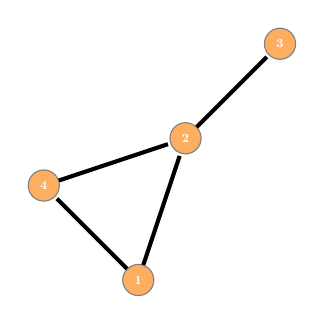
\begin{tikzpicture}[scale=.6]
         
        
           \tikzstyle{every edge}=[-,>=stealth',shorten >=1pt,auto,draw,line width=1.5pt]
           \tikzstyle{every state}=[draw, text=white,scale=0.95, transform shape]
          \tikzstyle{every state}=[draw=none,text=white,scale=0.75,  transform shape]
              \tikzstyle{every node}=[fill=orangeorg]

   \node[state, draw=black!50] (A1) at (2,0) {\textbf{1}};
    \node[state, draw=black!50] (A2) at (3,3) {\textbf{2}};
    \node[state, draw=black!50] (A3) at (5,5) {\textbf{3}};
    \node[state, draw=black!50] (A4) at (0,2) {\textbf{4}};

    \path (A1) edge [] (A2);
    \path (A1) edge  (A4);
    \path (A4) edge  (A2);
    \path (A2) edge  (A3);
 \end{tikzpicture}
 
 \smallskip
 Adjacency matrix:\\
 $\adj=\left(
\begin{array}{rrrrr}
0 & 1 & 0 & 1 \\ 
1 & 0 & 1 & 1 \\ 
0 & 1 & 0 & 0 \\ 
1 & 1 & 0 & 0 \\ 
\end{array}\right)
$
 \end{minipage}
 \begin{minipage}{0.49\linewidth}
  Bipartite network\\
  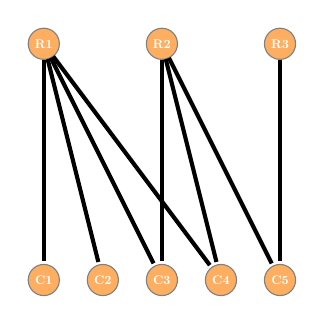
\begin{tikzpicture}[scale=.6]
         
        
           \tikzstyle{every edge}=[-,>=stealth',shorten >=1pt,auto,draw,line width=1.5pt]
           \tikzstyle{every state}=[draw, text=white,scale=0.95, transform shape]
          \tikzstyle{every state}=[draw=none,text=white,scale=0.75,  transform shape]
              \tikzstyle{every node}=[fill=orangeorg]

   \node[state, draw=black!50] (A1) at (0,5) {\textbf{R1}};
    \node[state, draw=black!50] (A2) at (2.5,5) {\textbf{R2}};
    \node[state, draw=black!50] (A3) at (5,5) {\textbf{R3}};
    \node[state, draw=black!50] (B1) at (0,0) {\textbf{C1}};
    \node[state, draw=black!50] (B2) at (1.25,0) {\textbf{C2}};
    \node[state, draw=black!50] (B3) at (2.5,0) {\textbf{C3}};
    \node[state, draw=black!50] (B4) at (3.75,0) {\textbf{C4}};
    \node[state, draw=black!50] (B5) at (5,0) {\textbf{C5}};
    \path (A1) edge [] (B1);
    \path (A1) edge  (B2);
    \path (A1) edge  (B3);
    \path (A1) edge  (B4);
    \path (A2) edge  (B3);
    \path (A2) edge  (B4);
    \path (A3) edge  (B5);
    \path (A2) edge  (B5);
 \end{tikzpicture}
 
 \smallskip
 Incidence matrix:\\
 $B=\left(
\begin{array}{rrrrr}
 1 &   1 &   1 &   1 &   0 \\ 
   0 &   0 &   1 &   1 &   1 \\ 
   0 &   0 &   0 &   0 &   1 \\  \end{array}\right)
$
 \end{minipage}


 \bigskip
 
 Network may also have weighted edges.
 
 
 %Adjacency matrix, simple, bipartite, distribution on edges...
 
\end{frame}




\begin{frame}
 \frametitle{Stochastic Block Model and Latent Block Model}

 Model on a simple network with $n$ nodes:
 
 \textbf{SBM:} \citemano{[NS01]}\\
 \begin{itemize}
 \item $K$ blocks of nodes sharing similar connection structure,
  \item $\bZ=(Z_1,\ldots,Z_n)$  independent latent variables s.t. $\P (Z_i=k)\overset{}{=} \pi_k$ for $k\in\{1,\ldots,K\}$ and $i\in\{1,\ldots,n\}$,
  \item $Y_{ij}|Z_i,Z_j\overset{ind}{\sim} \mathcal{F}(\alpha_{Z_i,Z_j})$ for all dyads $(i,j)$
 \end{itemize}

  

  \bigskip

  Model on a bipartite network with $n_1$ and $n_2$ nodes:

 \textbf{LBM:} \citemano{[GN10]}\\
 \begin{itemize}
 \item $K_1$ and $K_2$ blocks of nodes sharing similar connection structure,
 \item $\bZ^1=(Z^1_1,\ldots,Z^1_n)$ and $\bZ^2=(Z^2_1,\ldots,Z^2_m)$
 independent latent variables s.t.
 $\P(Z^1_i=k)=\pi^1_k$ for all $i\in\{1,\ldots,n\}$, $k\in\{1,\ldots,K_1\}$ and\\ $\P(Z^2_j=l)=\pi^2_l $ for all $j\in\{1,\ldots,m\}$, $l\in\{1,\ldots,K_2\}$
 \item $ Y_{ij}|Z^1_i,Z^2_j\overset{ind}{\sim} \mathcal{F}(\alpha_{Z^1_i,Z^2_j})$ for all dyads $(i,j)$.

 
 \end{itemize}
 
 

 %Graph to show how flexible they are to encompass a large variety of situation
\end{frame}


\begin{frame}
 \frametitle{Simulations under the SBM}
 \vspace{-.2cm}
 
\begin{figure}
%\hspace*{-1cm}
\begin{minipage}[c]{0.32\linewidth}
\tiny{$$\balpha=\left(
\begin{array}{rrr}
 0.70 & 0.09 & 0.09 \\ 
 0.09 & 0.70 & 0.09 \\ 
 0.09 & 0.09 & 0.70 \\ \end{array}\right)
$$}
\end{minipage}\hfill
\begin{minipage}[c]{0.32\linewidth}
\includegraphics[scale=.15]{Affiliation_graphe_with_colors.png}
\end{minipage}\hfill
\vspace{-.5cm}
\begin{minipage}[c]{0.32\linewidth}
\includegraphics[scale=.07]{Affiliation_reordered_adja_with_groups.png}
\end{minipage}
%\hspace*{-1cm}
\begin{minipage}[c]{0.32\linewidth}
\tiny{$$\balpha=\left(
\begin{array}{rrrr}
  0.70 & 0.70 & 0.70 & 0.70 \\ 
  0.70 & 0.70 & 0.70 & 0.09 \\ 
  0.70 & 0.70 & 0.09 & 0.09 \\ 
  0.70 & 0.09 & 0.09 & 0.09 \\ \end{array}\right)
$$}
\end{minipage}\hfill
\begin{minipage}[c]{0.32\linewidth}
\includegraphics[scale=.15]{Nested_graphe_with_colors.png}
\end{minipage}\hfill
\begin{minipage}[c]{0.32\linewidth}
\includegraphics[scale=.07]{Nested_reordered_adja_with_groups.png}
\end{minipage}
%\hspace*{-1cm}
\begin{minipage}[c]{0.32\linewidth}
\tiny{$$\balpha=\left(
\begin{array}{rrrr}
  0.09 & 0.70 & 0.09 & 0.09 \\ 
  0.70 & 0.09 & 0.09 & 0.09 \\ 
  0.09 & 0.09 & 0.09 & 0.70 \\ 
  0.09 & 0.09 & 0.70 & 0.09 \\ \end{array}\right)
$$}
\end{minipage}\hfill
\begin{minipage}[c]{0.32\linewidth}
\includegraphics[scale=.15]{Bipartite_graphe_with_colors.png}
\end{minipage}\hfill
\begin{minipage}[c]{0.32\linewidth}
\includegraphics[scale=.07]{Bipartite_reordered_adja_with_groups.png}
\end{minipage}
%\caption{Three particular binary network structures modeled through an SBM. First row corresponds to an assortative structure, second row to a nested structure, third row to a bipartite like structure. Left column gives the matrices of $\alpha=\P(Y_{ij}=1|Z_i,Z_j)$, middle column is a network plot where the colors correspond to the different blocks, right column is the reordered adjacency matrix with yellow square representing actual edges ($Y_{ij}=1$) and purple absence of edge.}
\label{figexSBM}
\end{figure}
\end{frame}





\begin{frame}
 \frametitle{Inference of the SBM}
 
 \textbf{Observed likelihood:}
 \begin{equation*}
 \label{eqLikobs}
 \log\ell(\btheta=(\balpha,\bpi);\bY)=\sum_{\bZ\in\{1,\ldots,K\}^n}  \log\ell_c(\btheta;\bY,\bZ)\,.
\end{equation*}
\smallskip

 \textbf{Difficulties:}
 \begin{itemize}
  \item Sum over $Z$ is then intractable as soon as either $n$ or $K$,
  \item $p(\bZ|\bY; \btheta)$ not tractable so EM algorithm not possible.
 \end{itemize}

 \smallskip
 \textbf{Solution:} Variational EM algorithm \citemano{[DPR8]} $\rightarrow$
 Replace $p(\bZ|\bY; \btheta)$ with
\begin{equation*}
 \label{eqVarDist}
 \mathcal{R}_{\bY,\btau}(\bZ) = \prod_{i=1}^{n}\prod_{k=1}^K (\tau_{ik})^{\ind_{Z_i = k}}, \quad \mbox{ where} \quad \tau_{ik} =\P_{\mathcal{R}_{\bY,\btau}}(Z_{i}  = k).
\end{equation*}

Maximizing alternatively in $\btheta$ and $\mathcal{R}$: 
\begin{equation*}
 \label{Ivar}
\mathcal{I}_{\btheta}(\mathcal{R}) = \log   \ell(  \btheta;\bY)  - \text{KL}[\mathcal{R}, \P(\cdot | \bY; \theta)].
 \end{equation*}

 
\end{frame}


\begin{frame}
 \frametitle{Selecting the number of blocks}
 Integrated Classification Likelihood 
 \citemano{[BCG00],[DPR8]}
 
 \bigskip
 
 
 \begin{equation*}\label{eq:ICL}
\text{ICL}(K) =\log  \ell_c( \hat \btheta_{K};\bY,\hat{\bZ})-  \text{pen}(K)
\end{equation*}
 where 
\begin{equation*}
\text{pen}(K) =   \frac{1}{2}\left\{ (K-1)\log(n)   +\left( K(K+1)/2 \right)  \log \left( n(n-1)/2 \right)\right\}\,,
\end{equation*}

for a binary undirected network.

\end{frame}








\subsection{Some contributions}



\begin{frame}
 \frametitle{Multilayer networks}
 
 
 \begin{itemize}
  \item Large variety of multilayer networks,
  \item SBM as a probabilistic generative model easy to extend to numerous cases.
  \item e.g. dynamic or spatial SBM (\citemano{[MM17],[MM19]}) or Topic SBM \citemano{[BLZ18]}.
 \end{itemize}

 \bigskip
 
 Our contributions
 
 \begin{itemize}
  \item Multiplex network \cite{barbillon2017stochastic,lazega2016effects},
   \item Multilevel network \cite{chabert2019stochastic},
  \item Multipartite network \cite{bar2018block}. 
 
 \end{itemize}

 Adaptation of the VEM algorithm and ICL criterion to select the numbers of blocks.
\end{frame}


\begin{frame}
 \frametitle{Multiplex network}
 
 In collaboration with A. Bar-Hen, S. Donnet and E. Lazega \cite{barbillon2017stochastic,lazega2016effects}.\\
 
 \bigskip
 
 Multiple relations between individuals: 
 $$
 \bY_{ij}|Z_i,Z_j \overset{ind}{\sim} \text{Bern}^Q((\alpha_{Z_i,Z_j}^w)_{ w}  ) \quad \text{with} \ \sum_{w}\alpha_{Z_i,Z_j}^w=1.
$$ 

 
 
 
 

\begin{figure}
    \centering
    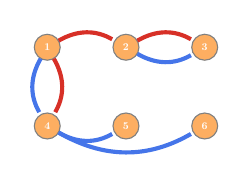
\begin{tikzpicture}[scale=.5]
         
        
           \tikzstyle{every edge}=[-,>=stealth',shorten >=1pt,auto,draw,line width=1.5pt]
           \tikzstyle{every state}=[draw, text=white,scale=0.95, transform shape]
          \tikzstyle{every state}=[draw=none,text=white,scale=0.75,  transform shape]
              \tikzstyle{every node}=[fill=orangeorg]

              
    \node[state, draw=black!50] (A1) at (0.5,3) {\textbf{1}};
    \node[state, draw=black!50] (A2) at (2.5,3) {\textbf{2}};
    \node[state, draw=black!50] (A3) at (4.5,3) {\textbf{3}};
    \node[state, draw=black!50] (A4) at (0.5,1) {\textbf{4}};
    \node[state, draw=black!50] (A5) at (2.5,1) {\textbf{5}};
    \node[state, draw=black!50] (A6) at (4.5,1) {\textbf{6}};
 
 
    \path (A1) edge [bend left,color=redorg] (A2);
    \path (A1) edge [bend left,color=redorg] (A4);
    \path (A1) edge [bend right,color=blueind] (A4);
    \path (A4) edge [bend right,color=blueind] (A5);
    \path (A4) edge [bend right,color=blueind] (A6);
    \path (A2) edge [bend left,color=redorg] (A3);
    \path (A2) edge [bend right,color=blueind] (A3);
    
    
    
     \end{tikzpicture}

    \caption{Illustration of a multiplex network. For each dyad, two kinds of link may exist. They are respectively displayed by red and blue edges. }
    \label{fig:plex}
\end{figure}         
 Model inference implemented in the \texttt{R} package: \texttt{blockmodels}.
 
 \smallskip
 
 \textbf{Application} to a network of French researchers in cancerology (advice relation and indirect relation through the labs of the researchers).
 
%  \smallskip
%  Application in Ecology of the same model in MW{+}16
 
\end{frame}


% \begin{frame}
%  \frametitle{Multiplex network application}
%  
%  
%  \textbf{Data:} French researchers in cancerology,
%  \begin{itemize}
%   \item Advice relations between researchers (R),
%   \item Institutional relations between their labs transferred to the researcher level as an undirect relation (L).
%  \end{itemize}
% 
%  
%  \vspace{-.5cm}
%  \begin{figure}[h!t!]
% \begin{center}
% \begin{tabular}{cc}
% \multicolumn{2}{c}{\includegraphics[width=3.5cm]{pR.pdf}}\vspace{-2cm}\\
% \includegraphics[width=3.5cm]{pRL0.pdf}&\includegraphics[width=3.5cm]{pRL1.pdf}
% \end{tabular}
%  \end{center}
%  \vspace{-.2cm}
%  \caption{Marginal and conditional probabilities for advice relation (R) between two researches in cancerology. 
%  L is an undirect relation through their labs.}
% \label{figRconnection}
%  \end{figure}
%  
%  \vspace{-.5cm}
% 
%  
% \end{frame}



\begin{frame}
 \frametitle{Multilevel network}
 In collaboration with S. Donnet and S.-C. Chabert-Liddell (Ph.D. Thesis) and E. Lazega \cite{chabert2019stochastic}.
 
 \vspace{-.8cm}
 \begin{figure}
    \centering
    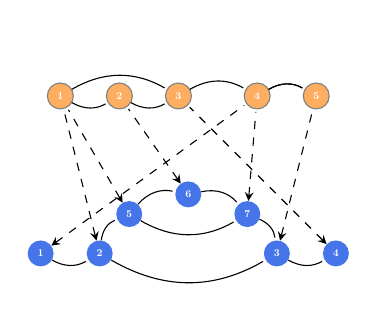
\begin{tikzpicture}[scale=.5]
          \node[fill=white, scale = 1] at (3, 4.5) {};  
          \tikzstyle{every edge}=[-,>=stealth',shorten >=1pt,auto,thin,draw]
          \tikzstyle{every state}=[draw, text=white,scale=0.95, transform shape]
    
         % Upper level
          \tikzstyle{every state}=[draw=none,text=white,scale=0.75,  transform shape]
          % premier cluster

          \tikzstyle{every node}=[fill=orangeorg]
          \node[state, draw=black!50] (LA1) at (0.5,3) {\textbf{1}};
          \node[state, draw=black!50] (LA2) at (2,3) {\textbf{2}};
          \node[state, draw=black!50] (LA3) at (3.5,3) {\textbf{3}}; 
          \tikzstyle{every node}=[fill=orangeorg]
          \node[state, draw=black!50] (LB1) at (5.5,3) {\textbf{4}};
          \node[state, draw=black!50] (LB2) at (7,3) {\textbf{5}};
          

          \path (LB1) edge [bend left] (LB2);
		  \path (LB1) edge [bend left] (LB2);
		  \path (LA3) edge [bend left]  (LB1);
 		  \path (LA1) edge [bend right] (LA2);
		  \path (LA2) edge [bend right] (LA3);
		  \path (LA1) edge [bend left]  (LA3);
          
          % Lower level
                    
          \tikzstyle{every node}=[fill={blueind},  double distance = 2pt]
          % premier cluster
          \node[state] (RA1) at (0, -1) {\textbf{1}};
          \node[state] (RA2) at (1.5, -1) {\textbf{2}};
          %2eme cluster
          \tikzstyle{every node}=[fill={blueind}, double distance = 2pt]
     	  \node[state] (RB1) at (6, -1) {\textbf{3}};
          \node[state] (RB2) at (7.5, -1) {\textbf{4}};
          \tikzstyle{every node}=[fill=blueind,  double distance = 2pt]
          % troisime cluster
          \node[state] (RC1) at (2.25,0) {\textbf{5}};
          \node[state] (RC2) at (3.75,.5) {\textbf{6}};
          \node[state] (RC3) at (5.25,0) {\textbf{7}};
          

          \tikzstyle{every edge}=[-,>=stealth', shorten >= 1pt, auto, thin, draw]
          \path (RA1) edge [bend right] (RA2);
          \path    (RB1)    edge     [bend    right]   (RB2) ;
          \path 	(RC1) edge [bend right]  (RC3)
            (RC1) edge [bend left] (RC2)
          	(RC2) edge [bend left] (RC3);
          % inter cluster
          \path 
          (RA2)    edge    [bend    right]    (RB1)
          (RC3) edge [bend left] (RB1)
          (RA2) edge [bend left] (RC1);
          
     %Interlevel link
          
		  \tikzstyle{every edge}=[dashed,>=stealth, <-,shorten >=1pt,auto,thin,draw]
		  \path (RA1) edge  (LB1);
		  \path (RA2) edge  (LA1);
		  \path (RC1) edge  (LA1);
		  \path (RC2) edge  (LA2);
		  \path (RC3) edge  (LB1);
		  \path (RB1) edge  (LB2);
		  \path (RB2) edge  (LA3);
          
        \end{tikzpicture}

  %  \caption{Illustration of a multilevel network following an MLVSBM. Inter-organizational level is on the top and inter-individual level is on the bottom.  The various shades of blue depict the blocks of individuals and the various shades of red depict the blocks of organizations.  The outer circles around the nodes of the individuals represent the blocks of the organizations they are affiliated to. The dashed links stand for the affiliations.}
    \label{fig:vuenetwork}
\end{figure}


\begin{itemize}
 %\item 2 levels: organizations and individuals,
 \item \color{orangeorg}Organizational level: \color{black} SBM for $(\bXL,\bZL)$,
 \item \color{blueind}Individual level: \color{black} SBM for $(\bXR,\bZR)$,
 \item Interlevel dependence $i\in\{1,\ldots,\nbr\}$, 
$k\in\{1,\ldots,\QR\}$,
$
     %\ZR{i}|  \ZL{j}, \aff_{ij} = 1\overset{ind}{\sim} \mathcal{M}(1,\gamma_{1\ZL{j}},\ldots,\gamma_{\QR\ZL{j}}).
       \P (\color{blueind}\ZR{i}\color{black}=k| \color{orangeorg} \ZL{j}\color{black}, \aff_{ij}=1)\overset{ind}{=} \gamma_{k\ZL{j}},
$ where $A$ is the affiliation matrix.
  \end{itemize}

  
  \smallskip
Implemented in S.-C. Chabert-Liddell's \texttt{R} package: \texttt{MLVSBM}.
 
 \smallskip
\textbf{Application} to a dataset of a program trade fair (Organizations = audiovisual firms, individuals = sales representatives ).
 
\end{frame}



\begin{frame}
 \frametitle{Generalized Multipartite Networks}
In collaboration with A. Bar-Hen and S. Donnet \cite{bar2018block}.
 
 
 \bigskip
 
 
 \begin{itemize}
  \item Pre-specified functional groups (colors of nodes),
  \item Looking for blocks within functional groups,
  \item Each network between 2 functional groups is either an SBM or an LBM.
 \end{itemize}

 
\begin{figure}
\centering

\begin{minipage}[t]{0.2\linewidth}
% Bipartite
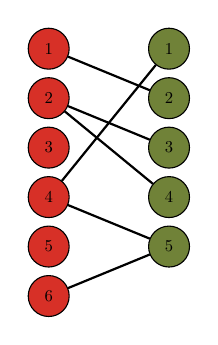
\begin{tikzpicture}[scale=.8,
  mynoder/.style={draw,circle,text width=0.5cm,fill = redorg,align=center,scale=0.6},
  mynodeg/.style={draw,circle,text width=0.5cm,align=center, fill = greenind,scale=0.6},
 ]

\node[mynoder] (R1) {$1$};
\node[mynoder, below=0.1 cm of R1] (R2) {$2$};
 \node[mynoder, below=0.1 cm of R2] (R3) {$3$};
 \node[mynoder, below=0.1 cm of R3] (R4) {$4$};
 \node[mynoder, below=0.1 cm of R4] (R5) {$5$};
 \node[mynoder, below=0.1 cm of R5] (R6) {$6$};
 
\node[mynodeg, right =1 cm of R1] (G1) {$1$};
\node[mynodeg, below=0.1 cm of G1] (G2) {$2$};
 \node[mynodeg, below=0.1 cm of G2] (G3) {$3$};
 \node[mynodeg, below=0.1 cm of G3] (G4) {$4$};
 \node[mynodeg, below=0.1 cm of G4] (G5) {$5$};

\path[thick]
(R1) edge (G2)
(R2) edge (G3) 
(R2) edge (G4)
(R4) edge (G1)
(R4) edge (G5)
(R6) edge (G5);

\end{tikzpicture}

    \end{minipage}\hfill
% Multipartite
\begin{minipage}[t]{0.5\linewidth}
\centering
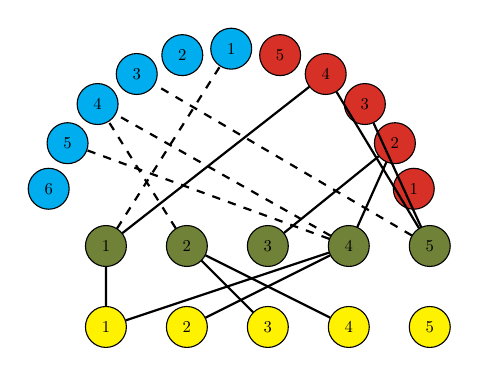
\begin{tikzpicture}[scale=.8,
  mynoder/.style={draw,circle,text width=0.5cm,fill = redorg,align=center,scale=0.6},
  mynodeg/.style={draw,circle,text width=0.5cm,align=center, fill = greenind,scale=0.6},
  mynodeb/.style={draw,circle,text width=0.5cm,align=center, fill=cyan,scale=0.6},
mynodey/.style={draw,circle,text width=0.5cm,align=center, fill=yellow,scale=0.6}
]
\foreach \a in {1,2,...,5}{
\node[mynoder] at ({90/6 * (\a)}:  3cm) (R\a) {$\a$};
}
\foreach \a in {1,2,...,6}{
\node[mynodeb] at ({90 + 90/6 * (\a-1)}:  3cm) (B\a) {$\a$};
}
 

\node[mynodeg, below right  = 0.5 cm of B6] (G1) {$1$};
\node[mynodeg, right =0.5  cm of G1] (G2) {$2$};
 \node[mynodeg,right =0.5  cm of G2] (G3) {$3$};
 \node[mynodeg,right =0.5  cm of  G3] (G4) {$4$};
 \node[mynodeg, right =0.5  cm of G4] (G5) {$5$};

\node[mynodey, below = 0.5 cm of G1] (Y1) {$1$};
\node[mynodey, right =0.5  cm of Y1] (Y2) {$2$};
 \node[mynodey,right =0.5  cm of Y2] (Y3) {$3$};
 \node[mynodey,right =0.5  cm of  Y3] (Y4) {$4$};
 \node[mynodey, right =0.5  cm of Y4] (Y5) {$5$};
 \path[thick]
(R2) edge (G3) 
(R3) edge (G5) 
(R2) edge (G4)
(R4) edge (G1)
(R4) edge (G5);



\path[thick]
(G1) edge [dashed] (B1)
(G2) edge [dashed] (B4)
(G4) edge [dashed] (B4)
(G4) edge [dashed] (B5)
(G5) edge [dashed] (B3);

\path[thick]
(G1) edge (Y1)
(G2) edge (Y4) 
(G2) edge (Y3)
(G4) edge (Y2)
(G4) edge (Y1);



\end{tikzpicture}
    \end{minipage}\hfill
\begin{minipage}[t]{0.3\linewidth}
\centering
\begin{tikzpicture}[scale=.8,
  mynoder/.style={draw,circle,text width=0.5cm,fill = redorg,align=center,scale=0.6},
  mynodeg/.style={draw,circle,text width=0.5cm,align=center, fill = greenind,scale=0.6},
  mynodeb/.style={draw,circle,text width=0.5cm,align=center, fill=redorg,scale=0.6}
]
%
%\node[mynoder] (R1) {$1$};
%\node[mynoder, right=0.1 cm of R1] (R2) {$2$};
% \node[mynoder, right=0.1 cm of R2] (R3) {$3$};
% \node[mynoder, right=0.1 cm of R3] (R4) {$4$};
% \node[mynoder, right=0.1 cm of R4] (R5) {$5$};
% \node[mynoder, right=0.1 cm of R5] (R6) {$6$};
 
\node[mynodeg, below =1 cm of R1] (G1) {$1$};
\node[mynodeg, right=0.1 cm of G1] (G2) {$2$};
 \node[mynodeg, right = 0.1 cm of G2] (G3) {$3$};
 \node[mynodeg, right=0.1 cm of G3] (G4) {$4$};
 \node[mynodeg, right=0.1 cm of G4] (G5) {$5$};

\node[mynodeb, below =1 cm of G1] (B1) {$1$};
\node[mynodeb, right =0.1 cm of B1] (B2) {$2$};
 \node[mynodeb, right =0.1 cm of B2] (B3) {$3$};
 \node[mynodeb, right =0.1 cm of B3] (B4) {$4$};
 \node[mynodeb, right=0.1 cm of B4] (B5) {$5$};
 \node[mynodeb, right=0.1 cm of B5] (B6) {$6$};

%\path[thick]
%(R1) edge (G2)
%(R2) edge (G3) 
%(R2) edge (G4)
%(R4) edge (G1)
%(R4) edge (G5)
%(R6) edge (G5);


\path[thick]
(G1) edge (B1)
(G2) edge (B4) 
(G2) edge (B2)
(G4) edge (B6)
(G4) edge (B3)
(G5) edge (B6);


\path[->] 
(B1) edge [bend right = 70] (B2)
(B3) edge [bend right = 70] (B5)
(B5) edge [bend left = 80] (B1)
(B6) edge [bend left = 70] (B4);
\end{tikzpicture}
    \end{minipage}

\caption{Illustrations of bipartite (left), multipartite (center) and generalized multipartite networks (right). The colors stand for the different functional groups. }
\label{fig:schema bipar}
\end{figure}

 
 Implemented in an \texttt{R} package: \texttt{GREMLINS}.

 
\end{frame}


\begin{frame}
 \frametitle{Application in Ecology}
 \textbf{Dataset:} Interaction between plants and $\{\text{pollinators,ants,birds}\}$  \citemano{[DLRJ+16]}
 
\begin{figure}[ht]
\centering
   \includegraphics[scale=0.55]{dattilo.png}
   \caption{Mesoscopic view. Size of nodes is prop to number of entities per block and widths of edges prop to probabilities of connection between blocks}% of dataset 1. Nodes stand for the inferred blocks, their size are proportional to the size of the blocks
   %and the width of the edges are proportional to the probability of connection between/within blocks. Edges corresponding to probabilities of connection lower than 0.01 are not plotted.}
   \label{fig:estim dattilo}
\end{figure}
\end{frame}




\begin{frame}
 \frametitle{Inferring the SBM from an observed network (Missing data)}
 In collaboration with J. Chiquet and T. Tabouy (Ph.D. Thesis) \cite{tim}.
 
 \medskip
 \textbf{Observation of a network}:
  $n\times n$ binary matrix $\bR$ such that $R_{ij}=1$ if $Y_{ij}$ is observed, $R_{ij}=0$ otherwise ($Y_{ij}=\texttt{NA}$).
  
  \medskip
  \textbf{Observation process:} \citemano{[Rub76]} MCAR, MAR or NMAR?
  \begin{figure}
  \centering
  \begin{tabular}{@{}c@{\hspace{5em}}c@{}}
    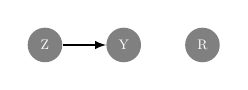
\begin{tikzpicture}[scale=.5]
      \tikzstyle{every edge}=[-,>=stealth',shorten >=1pt,auto,thin,draw]
      \tikzstyle{every state}=[draw=none,text=white, font=\normalsize, transform shape]
      \tikzstyle{every node}=[fill=white!50!black]
      \node[state] (Z) at (0,0) {Z};
      \node[state] (Y) at (2,0) {Y};
      \node[state] (R) at (4,0) {R};
      \draw[->,>=latex] (Z) -- (Y);
      %    \draw[->,>=latex] (Y) -- (R);
    \end{tikzpicture}
    &
    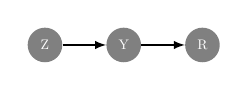
\begin{tikzpicture}[scale=.5]
      \tikzstyle{every edge}=[-,>=stealth',shorten >=1pt,auto,thin,draw]
      \tikzstyle{every state}=[draw=none,text=white, font=\normalsize, transform shape]
      
      \tikzstyle{every node}=[fill=white!50!black]
      \node[state] (Z) at (0,0) {Z};
      \node[state] (Y) at (2,0) {Y};
      \node[state] (R) at (4,0) {R};
      
      \draw[->,>=latex] (Z) -- (Y);
      \draw[->,>=latex] (Y) -- (R);
    \end{tikzpicture}
    \\
    \scriptsize (MCAR) & \scriptsize (MAR or NMAR) \\[3ex]
    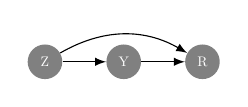
\begin{tikzpicture}[scale=.5]
        
        \tikzstyle{every edge}=[-,>=stealth',shorten >=1pt,auto,thin,draw]
      \tikzstyle{every state}=[draw=none,text=white, font=\normalsize, transform shape]
        
        \tikzstyle{every node}=[fill=white!50!black]
        \node[state] (Z) at (0,0) {Z};
        \node[state] (Y) at (2,0) {Y};
        \node[state] (R) at (4,0) {R};
        
        \draw[->,>=latex] (Z) -- (Y);
        \draw[->,>=latex] (Y) -- (R);
        \draw[->,>=latex] (Z) to[bend left] (R);
        
      \end{tikzpicture}
    &
      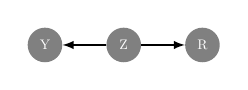
\begin{tikzpicture}[scale=.5]
        
        \tikzstyle{every edge}=[-,>=stealth',shorten >=1pt,auto,thin,draw]
      \tikzstyle{every state}=[draw=none,text=white, font=\normalsize, transform shape]
        \tikzstyle{every node}=[fill=white!50!black]
        \node[state] (Z) at (0,0) {Z};
        \node[state] (Y) at (-2,0) {Y};
        \node[state] (R) at (2,0) {R};
        
        \draw[->,>=latex] (Z) -- (Y);
        \draw[->,>=latex] (Z) -- (R);
      \end{tikzpicture}
    \\
    \scriptsize (NMAR) & \scriptsize (NMAR) \\
  \end{tabular}    
  \label{fig:DAGs}
\end{figure}

\medskip
\textbf{Inference under M(C)AR scheme:} Likelihood on the observed data.
  
 % \medskip

  
\end{frame}


\begin{frame}
 \frametitle{Inference under NMAR scheme}
 
 Need for accounting for the complete likelihood where we have missing data ($\MAM$) and latent variables $\bZ$
 
 Variational distribution on $(\MAM,\bZ)$ in the VEM algorithm:
 \begin{equation*}
  \label{eq:approx_nmar}
  \mathcal{R}_{(\MAM,\bZ)} = \mathcal{R}_{(\MAM)}\cdot \mathcal{R}_{(\bZ)}
  =  \prod_{(i,j), Y_{ij}=NA} \nu_{ij}^{Y_{ij}}(1-\nu_{ij})^{1-Y_{ij}}\cdot \prod_{i=1}^n \prod_{k=1}^K (\tau_{ik})^{\ind_{Z_i = k}},
\end{equation*}
where 
\begin{itemize}
 \item $\nu_{ij}$s and $\tau_{ik}$s parameters to be optimized in the VE step,
 \item $\tau_{ik}$ is almost generic,
 \item $\nu_{ij}$ is specific to the sampling design.
\end{itemize}


\bigskip
\textbf{Contributions:}
\begin{itemize}
 \item Derived variational steps for some NMAR sampling schemes,
 \item Importance of accounting for sampling illustrated on synthetic and real data,
 \item Implementation in an \texttt{R} package \texttt{missSBM} \cite{missSBM}.
\end{itemize}


 
\end{frame}




\subsection{Perspectives on networks}


\begin{frame}
 \frametitle{Sampling in ecological network}
In collaboration with C. Fontaine and \'E. Thébault.
 
 
 \begin{itemize}
  \item Observation process: only $Y_{ij}=1$ are actually observed all other are \texttt{NA}, 
  
  
  \item Estimation of completness of a sampling from accumulation curves or richness estimators.
 
 
 
 \includegraphics[scale=.2]{completude.pdf}
 
 \item Adapt to handle data from citizen science.

 
  \item Master Internship of Thomas Cortier.

\item  Ph.D. Thesis proposition: half-grant from ANR Econet.

 \end{itemize}

\end{frame}

% 
% \subsection{Perspectives}
% \begin{frame}
%  \frametitle{Robustness}
%  
% \end{frame}






\begin{frame}
 \frametitle{Other perspectives on networks}
 
 \begin{itemize}
 \item Computation of ecological descriptors of a network such as robustness (S.-C. Chabert Liddell's ongoing work) derived from an LBM, enabling comparison of renormalized networks.
 
 \smallskip
  \item \texttt{R} Package \texttt{sbm} (with J. Chiquet and S. Donnet): a unique package to %\color{gray}\sout{rule them all} \color{black} 
  interface the different packages inferring SBM, coming with common features such as representation, data manipulation...
  
   \smallskip

   
   \item Assessing the role of social organization on cultivated biodiversity and diversity of domestic animals: interdisciplinary research groups \textsc{Mires} group, \textsc{Resodiv} GDR and \textsc{Pastodiv} ANR.
   
   
%   \item \textsc{Mires} group: Assessing the impact of social interaction between farmers on the cultivated biodiversity. 
%   
%    \smallskip
% 
%   \item \textsc{Resodiv} GDR: Circulation of seeds, knowledge, animals.
%   
%   \item  \textsc{Pastodiv} ANR understanding of the dynamics of domestic animals diversity through pastoral practices.
 \end{itemize}

 
\end{frame}


\section*{Many}
\begin{frame}
\frametitle{Many Thanks}

%citer collaborators
 \textbf{MIA Paris} Julien Chiquet, Sophie Donnet, Marie-Pierre Étienne, Jean-Benoist Léger, Tristan Mary-Huard, Éric Parent, Stéphane Robin, Loïc Schwaller
 
 
 \textbf{SAMSI} Evan Baker, Jim Berger, Anabel Forte, Robert Gramacy, David Higdon, Pulong Ma, Rui Paulo, Bruce Pitman, Jerry Sacks
 
 
 \textbf{Elsewhere} Avner Bar-Hen, Célia Barthélémy, Sophie Caillon, Matthieu Chiodetti, Sonia Kéfi, Andrew Flachs, Colin Fontaine, Merlin Keller, Vanesse Labeyrie, Adeline Leclercq-Samson, Jean-Michel Marin, François Massol, Luc Perreault, Matthieu Salpeteur, Elisa Thébault, Mathieu Thomas, Nicolas Verzelen, Jean Wencélius
 
 
 \textbf{Co-supervised Master or Ph.D. students and Post-doc fellows}
 Emmanuelle Blanc, Mathieu Carmassi, Thomas Cortier, Marie Courbariaux, Saint-Clair Chabert-Liddell, Sixtine de Cussac, Guillaume Damblin, Kaniav Kamary, Jordi Ferrer-Savall, Timothée Tabouy
 
 ...
 
 
 \includegraphics[scale=.1]{vieuxCB.jpg}
 \includegraphics[scale=.15]{samsi.jpeg}
 \includegraphics[scale=.18]{nouvagro.jpg}
 
\end{frame}



%\begin{frame}

\section*{References}

\tiny
\bibliographystyle{abbrv}
\bibliography{refHDR}
 
%\end{frame}




%\begin{frame}
 \frametitle{References}
\begin{thebibliography}{NS01}

\bibitem[BCG00]{biernacki2000}
C.~Biernacki, G.~Celeux, and G.~Govaert.
\newblock Assessing a mixture model for clustering with the integrated
  completed likelihood.
\newblock {\em Pattern Analysis and Machine Intelligence, IEEE Transactions
  on}, 22(7):719--725, Jul 2000.

\bibitem[BLZ18]{bou}
C.~Bouveyron, P.~Latouche, and R.~Zreik.
\newblock The stochastic topic block model for the clustering of vertices in
  networks with textual edges.
\newblock {\em Statistics and Computing}, 28(1):11--31, 2018.

\bibitem[DLRJ{{+}}16]{Dattilo}
W.~D{\'a}ttilo, N.~Lara-Rodr{\'\i}guez, P.~Jordano, P.~R. Guimar{\~a}es, J.~N.
  Thompson, R.~J. Marquis, L.~P. Medeiros, R.~Ortiz-Pulido, M.~A.
  Marcos-Garc{\'\i}a, and V.~Rico-Gray.
\newblock Unravelling {D}arwin{\textquoteright}s entangled bank: architecture
  and robustness of mutualistic networks with multiple interaction types.
\newblock {\em Proceedings of the Royal Society of London B: Biological
  Sciences}, 283(1843), 2016.

\bibitem[DPR08]{daudin2008mixture}
J.-J. Daudin, F.~Picard, and S.~Robin.
\newblock A mixture model for random graphs.
\newblock {\em Statistics and computing}, 18(2):173--183, 2008.

\bibitem[GN10]{govaert2010latent}
G.~Govaert and M.~Nadif.
\newblock Latent block model for contingency table.
\newblock {\em Communications in Statistics—Theory and Methods},
  39(3):416--425, 2010.

\bibitem[JSW98]{Jones98}
D.R. Jones, M.~Schonlau, and W.J. Welch.
\newblock Efficient global optimization of expensive black-box functions.
\newblock {\em Journal of Global Optimization}, 13(4):455--492, 1998.

\bibitem[KL04]{kuhn2004coupling}
E.~Kuhn and M.~Lavielle.
\newblock Coupling a stochastic approximation version of {EM} with an {MCMC}
  procedure.
\newblock {\em ESAIM: Probability and Statistics}, 8:115--131, 2004.

\bibitem[KMRR14]{kamary2014testing}
K.~Kamary, K.~Mengersen, C.~P. Robert, and J.~Rousseau.
\newblock Testing hypotheses via a mixture estimation model.
\newblock {\em arXiv preprint arXiv:1412.2044}, 2014.

\bibitem[KMW{+}16]{kefi2016structured}
S. K{\'e}fi, V. Miele, E.A. Wieters, S.A.Navarrete, and E.L.
  Berlow.
\newblock How structured is the entangled bank? the surprisingly simple
  organization of multiplex ecological networks leads to increased persistence
  and resilience.
\newblock {\em PLoS biology}, 14(8):e1002527, 2016.


\bibitem[KO01]{kennedy2001bayesian}
M.~C. Kennedy and A.~O'Hagan.
\newblock Bayesian calibration of computer models.
\newblock {\em Journal of the Royal Statistical Society: Series B (Statistical
  Methodology)}, 63(3):425--464, 2001.

\bibitem[LBH{{+}}06]{linketal2006}
C. Linkletter, D. Bingham, N. Hengartner, D. Higdon, and
  K.Q. Ye.
\newblock Variable selection for {Gaussian} process models in computer
  experiments.
\newblock {\em Technometrics}, 48(4):478--490, 2006.

\bibitem[LM19]{longepierre2019consistency}
L.~Longepierre and C.~Matias.
\newblock Consistency of the maximum likelihood and variational estimators in a
  dynamic stochastic block model.
\newblock {\em Electronic Journal of Statistics}, 13(2):4157--4223, 2019.

\bibitem[MM17]{matiasmiele}
C.~Matias and V.~Miele.
\newblock Statistical clustering of temporal networks through a dynamic
  stochastic block model.
\newblock {\em Journal of the Royal Statistical Society: Series B (Statistical
  Methodology)}, 79(4):1119--1141, 2017.

\bibitem[NS01]{nowickiSnijders2001}
K.~Nowicki and T.~A.~B. Snijders.
\newblock Estimation and prediction for stochastic blockstructures.
\newblock {\em Journal of the American Statistical Association},
  96(455):1077--1087, 2001.

\bibitem[Rub76]{Rubin1976}
D.~B. Rubin.
\newblock Inference and missing data.
\newblock {\em Biometrika}, 63(3):581--592, 1976.

\bibitem[SWMW89]{sacks1989design}
J. Sacks, W.J. Welch, T.J. Mitchell, and H.P. Wynn.
\newblock Design and analysis of computer experiments.
\newblock {\em Statistical science}, pages 409--423, 1989.


\end{thebibliography}
%\end{frame}



\end{document}
